% fig03_pipeline.tex — TikZ stage-flow diagram for the §Full Pipeline section.
% Compiled by the paper Makefile via `make figures` (pdflatex on the snippet).
% Relabel the seven nodes for your domain; the tier emoji column is intentionally
% inside the node so the diagram is independently readable (no need to cross-ref
% the §Full Pipeline table).
%
% Manual single-shot compile (debug):
%   pdflatex -interaction=nonstopmode -halt-on-error fig03_pipeline.tex
\documentclass[tikz,border=4pt]{standalone}
\usetikzlibrary{positioning,arrows.meta,shapes.geometric}
\begin{document}
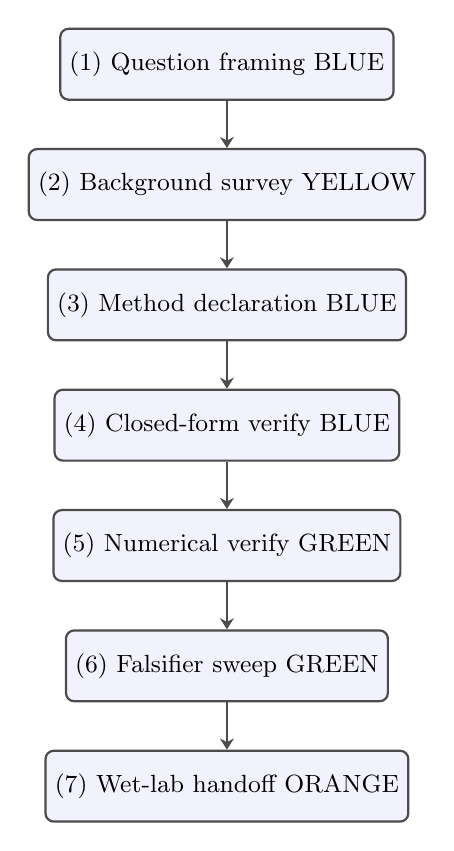
\begin{tikzpicture}[
  font=\small,
  stage/.style = {
    rectangle, rounded corners=3pt, draw=black!70, thick,
    minimum width=3.4cm, minimum height=0.9cm, align=left,
    fill=blue!5,
  },
  arrow/.style = {-{Stealth[length=4pt,width=5pt]}, thick, draw=black!70},
  node distance=0.6cm and 0.7cm,
]
  \node[stage] (s1) {(1) Question framing    \hfill BLUE};
  \node[stage, below=of s1] (s2) {(2) Background survey   \hfill YELLOW};
  \node[stage, below=of s2] (s3) {(3) Method declaration  \hfill BLUE};
  \node[stage, below=of s3] (s4) {(4) Closed-form verify  \hfill BLUE};
  \node[stage, below=of s4] (s5) {(5) Numerical verify    \hfill GREEN};
  \node[stage, below=of s5] (s6) {(6) Falsifier sweep     \hfill GREEN};
  \node[stage, below=of s6] (s7) {(7) Wet-lab handoff     \hfill ORANGE};

  \draw[arrow] (s1) -- (s2);
  \draw[arrow] (s2) -- (s3);
  \draw[arrow] (s3) -- (s4);
  \draw[arrow] (s4) -- (s5);
  \draw[arrow] (s5) -- (s6);
  \draw[arrow] (s6) -- (s7);
\end{tikzpicture}
\end{document}
